\documentclass[a4paper,12pt]{article}
\usepackage[a4paper,margin=1in]{geometry}
\usepackage{graphicx}
\usepackage[dvipsnames]{xcolor}
\usepackage{fancyhdr}
\usepackage{titlesec}
\usepackage{enumitem}
\usepackage{amsmath}
\usepackage{caption}
\usepackage{subcaption}
\usepackage{setspace}

% Define NCERT Blue
\definecolor{ncertblue}{RGB}{0,153,204}
\begin{document}
% Header layout
\begin{minipage}{0.6\textwidth}
   \vspace{-9em} 
\includegraphics[height=1.8cm]{iiitbcomet.jpg} % Replace with actual logo image
\end{minipage}
\hfill
\begin{minipage}{0.35\textwidth}
\raggedleft
\vspace{-9em}
\textbf{Name:} K.Alekya \\
\textbf{Batch:} COMETFWC024 \\
\textbf{Date:} 16 May 2025
\end{minipage}
\pagestyle{fancy}
\fancyhf{}
\vspace{-1em}

\cfoot{\textcolor{black}{Reprint 2025-26}}
\renewcommand{\headrulewidth}{0.4pt}
\renewcommand{\headrule}{\hbox to\headwidth{\color{ncertblue}\leaders\hrule height \headrulewidth\hfill}}
\setlength{\parindent}{0pt}
Also, it is given that
\[
\angle PST = \angle PRQ \hfill (2)
\]
So,  
\[
\angle PRQ = \angle PQR \quad \text{[From (1) and (2)]}
\]
Therefore,  
\[
PQ = PR \quad \text{(Sides opposite the equal angles)}
\]
i.e., \quad PQR is an isosceles triangle.
\vspace{1em}

\begin{center}
\textcolor{ncertblue}{\textbf{EXERCISE 6.2}}
\end{center}

\textbf{1.} In Fig. 6.17, (i) and (ii), DE $\parallel$ BC. Find EC in (i) and AD in (ii).

% Side-by-side images for Fig. 6.17
\begin{figure}[h!]
\centering
\begin{subfigure}{0.45\textwidth}
    \centering
    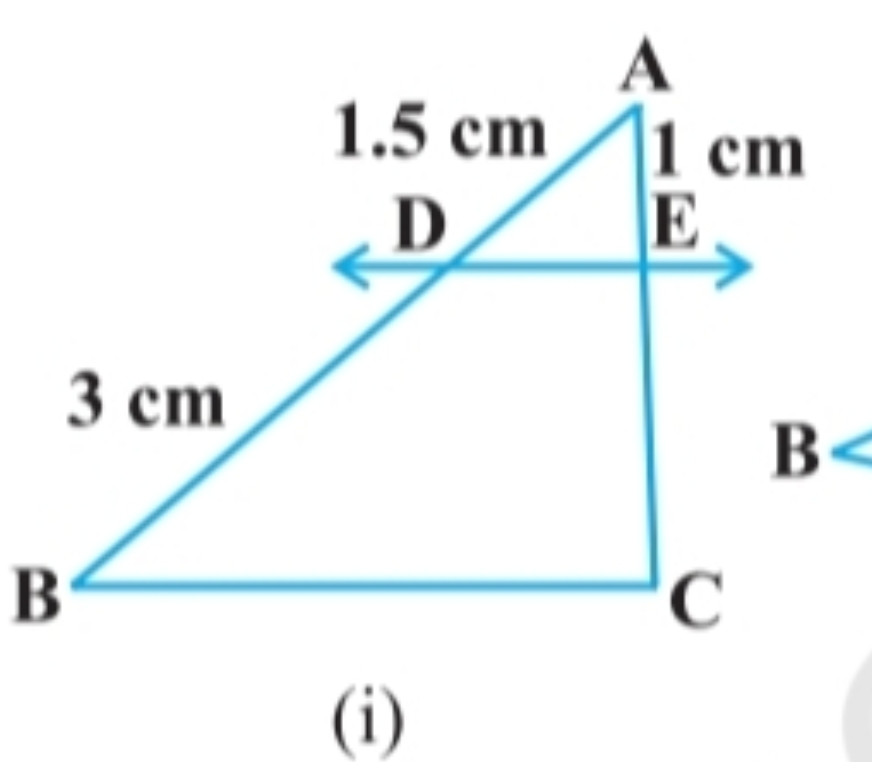
\includegraphics[width=0.9\textwidth]{a0.jpg}
    \caption*{(i)}
\end{subfigure}
\hfill
\begin{subfigure}{0.45\textwidth}
    \centering
    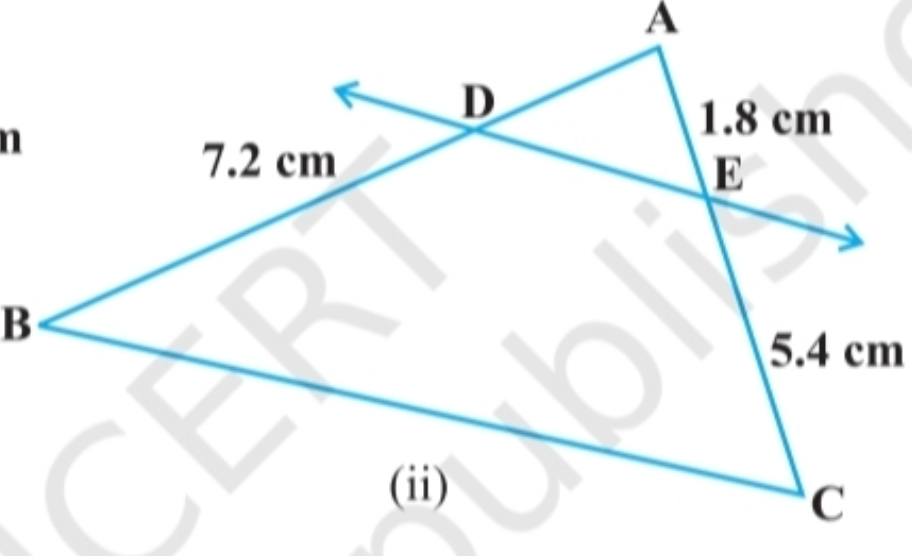
\includegraphics[width=0.9\textwidth]{a1.jpg}
    \caption*{(ii)}
\end{subfigure}
\end{figure}

\vspace{1em}

\textbf{2.} E and F are points on the sides PQ and PR respectively of a $\triangle PQR$. For each of the following cases, state whether EF $\parallel$ QR :

\begin{enumerate}[label=(\roman*)]
\item PE = 3.9 cm, EQ = 3 cm, PF = 3.6 cm and FR = 2.4 cm  
\item PE = 4 cm, QE = 4.5 cm, PF = 8 cm and RF = 9 cm  
\item PQ = 1.28 cm, PR = 2.56 cm, PE = 0.18 cm and PF = 0.36 cm  
\end{enumerate}

\vspace{1em}

\textbf{3.} In Fig. 6.18, if LM $\parallel$ CB and LN $\parallel$ CD, prove that  
\[
\frac{AM}{AB} = \frac{AN}{AD}
\]


\hspace{25em}
\vspace{-15em}
\vspace{5em}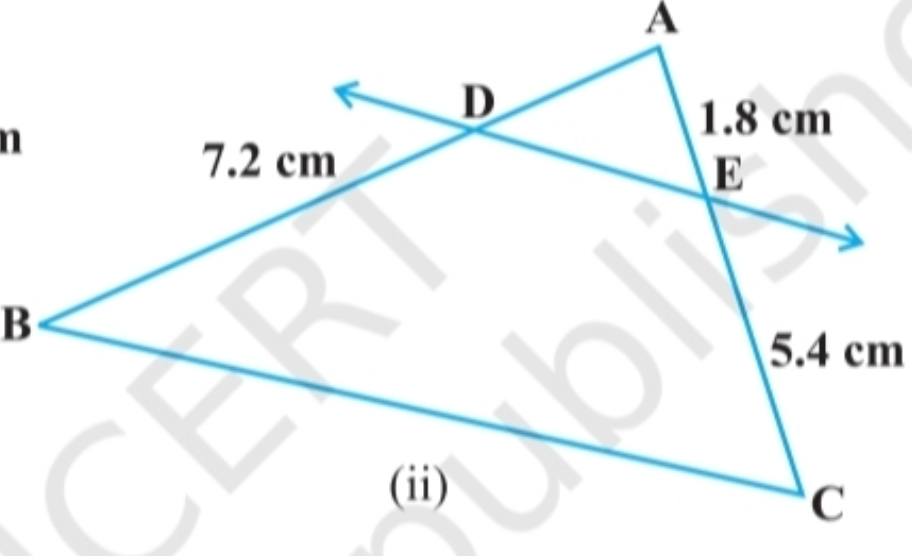
\includegraphics[width=0.4\textwidth]{a2.jpg}


\vspace{1em}

\textbf{4.} In Fig. 6.19, DE $\parallel$ AC and DF $\parallel$ AE. Prove that  
\[
\frac{BF}{FE} = \frac{BE}{EC}
\]

\titleformat{\section}{\color{ncertblue}\bfseries\large}{}{0em}{}
\titleformat{\subsection}[runin]{\bfseries}{}{0em}{}[.]
\pagestyle{fancy}
\fancyhf{}
\lhead{\textcolor{ncertblue}{\textbf{TRIANGLES}}}
\rhead{\textcolor{ncertblue}{\textbf{85}}}
\cfoot{\textcolor{black}{Reprint 2025-26}}

\renewcommand{\headrulewidth}{0.4pt}
\renewcommand{\headrule}{\hbox to\headwidth{\color{ncertblue}\leaders\hrule height \headrulewidth\hfill}}
\setlength{\parindent}{0pt}
\onehalfspacing

% Q5 + Fig 6.20 side-by-side
\begin{minipage}[t]{0.6\textwidth}
\vspace{-12em}
\textbf{5.} In Fig. 6.20, DE $\parallel$ OQ and DF $\parallel$ OR.  
Show that EF $\parallel$ QR.
\end{minipage}
\begin{minipage}[t]{0.38\textwidth}
\centering
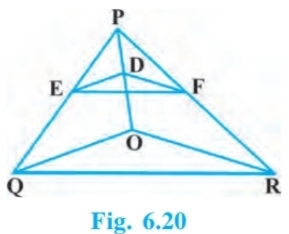
\includegraphics[width=\linewidth]{a3.jpg}\\
\end{minipage}

\vspace{2em}

% Q6 + Fig 6.21 side-by-side
\begin{minipage}[t]{0.6\textwidth}
\vspace{-22em}
\textbf{6.} In Fig. 6.21, A, B and C are points on OP, OQ and OR respectively  
such that AB $\parallel$ PQ and AC $\parallel$ PR.  
Show that BC $\parallel$ QR.
\end{minipage}
\begin{minipage}[t]{0.38\textwidth}
\centering
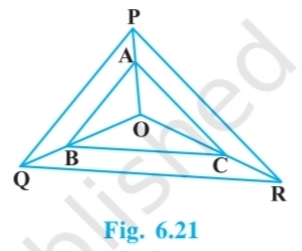
\includegraphics[width=\linewidth]{a4.jpg}\\
\end{minipage}

\vspace{-17em}

% Questions 7 to 10 without images
\textbf{7.} Using Theorem 6.1, prove that a line drawn\\ through  
the mid-point of one side of a triangle parallel\\ to another side  
bisects the third side. (Recall that you\\ have proved it in Class IX.)

\vspace{1em}

\textbf{8.} Using Theorem 6.2, prove that the line joining the \\ 
mid-points of any two sides of a triangle is parallel to  \\
the third side. (Recall that you have done it in Class IX.)

\vspace{1em}

\textbf{9.} ABCD is a trapezium in which AB $\parallel$ DC and its  \\
diagonals intersect each other at the point O. Show\\ that  
\[
\frac{AO}{BO} = \frac{CO}{DO}
\]

\vspace{1em}

\textbf{10.} The diagonals of a quadrilateral ABCD intersect each  
other at the point O such that  
\[
\frac{AO}{BO} = \frac{CO}{DO}
\]
Show that ABCD is a trapezium.

\vspace{-1em}

% Section 6.4
\section*{6.4 \hspace{0.5em} Criteria for Similarity of Triangles}

In the previous section, we stated that two triangles are similar,  
if (i) their corresponding angles are equal and  
(ii) their corresponding sides are in the same ratio (or proportion).

That is, in $\triangle ABC$ and $\triangle DEF$, if
\begin{itemize}
  \item[(i)] $\angle A = \angle D$, $\angle B = \angle E$, $\angle C = \angle F$
  \item[(ii)] $\dfrac{AB}{DE} = \dfrac{BC}{EF} = \dfrac{CA}{FD}$
\end{itemize}
then the two triangles are similar (see Fig. 6.22).
\end{document}
